\label{CCS811}

Wir haben den in Abbildung ...  zu sehenden CCS811-Sensor verwendet da er einige Vorteile mit sich bringt. Er ist ein digitaler \ac{MOX}-Gassensor mit einem extrem geringen Stromverbrauch. Wie in Abbildung \ref{fig:ccs811Blockdiagramm} zu sehen ist, besitzt er einen \ac{AD}-Wander und eine I$^2$C-Schnittstelle, was dem Entwickler eine leichte Soft- und Hardware Integration bietet. Zudem soll er eine Lebenszeit von über 5 Jahren nachweisen. \cite[vgl. S. 1]{amsAG.2016} \\

%\begin{figure}[!hbt]
%	\centering
%	\includegraphics[width=0.9\linewidth]{Images/CCS811Gassensor}
%	\caption{CCS811-\ac{MOX}-Gassensor}
%	\label{fig:CCS811-Bild}
%\end{figure}

Der CO2-Sensor ist über den Pins SDA und SCL mit dem Arduino verbunden. Pin 7 ist dabei auf Masse kurzgeschlossen. Die restlichen Pins werden in unserem Projekt nicht benötigt.

\begin{figure}[!hbt]
	\centering
	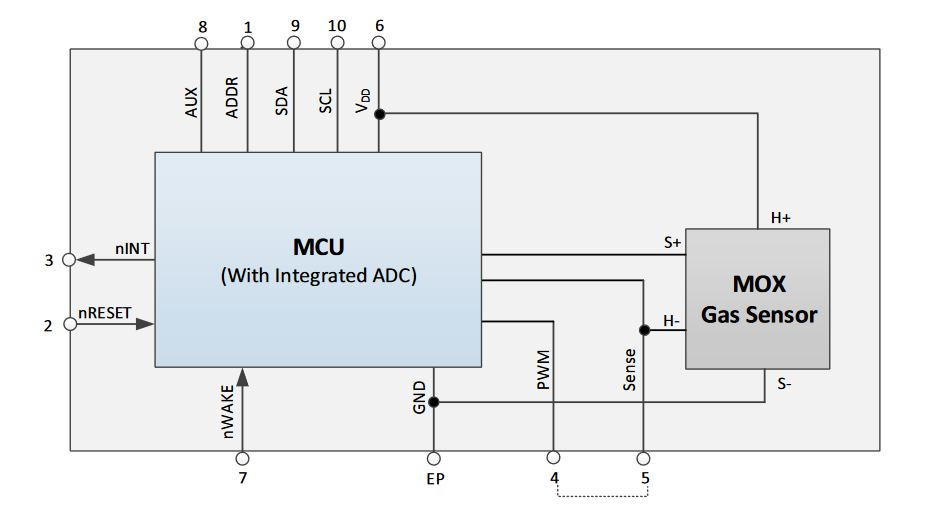
\includegraphics[width=0.9\linewidth]{Images/ccs811Blockdiagramm}
	\footnotesize{Quelle: \cite[S. 3]{amsAG.2016}}
	\caption{CCS811 Blockdiagramm}
	\label{fig:ccs811Blockdiagramm}
\end{figure}

Der Abruf von Messdaten auf dem I$^2$C erfolgt über das Master-Slave Prinzip. Dabei nimmt der Arduino die Rolle des Masters, und der CO\textsubscript{2}-Sensor die des Slaves ein. Das bedeutet, der CCS811 darf nur Informationen senden, wenn er vom Arduino die Aufforderung bekommen hat. \\
Um an die richtigen Daten des Sensors zu gelangen, muss der Arduino in unserem Projekt die ersten beiden Bytes auslesen, da diese die nötigen Informationen über den CO\textsubscript{2}-Gehalt der Luft zu Verfügung stellen. Die restlichen Bytes werden in unserem Projekt nicht ausgelesen, da wir für diese keine Verwendung haben.

\begin{center}
	
	\begin{figure}[!hbt]
		
		\centering
		
		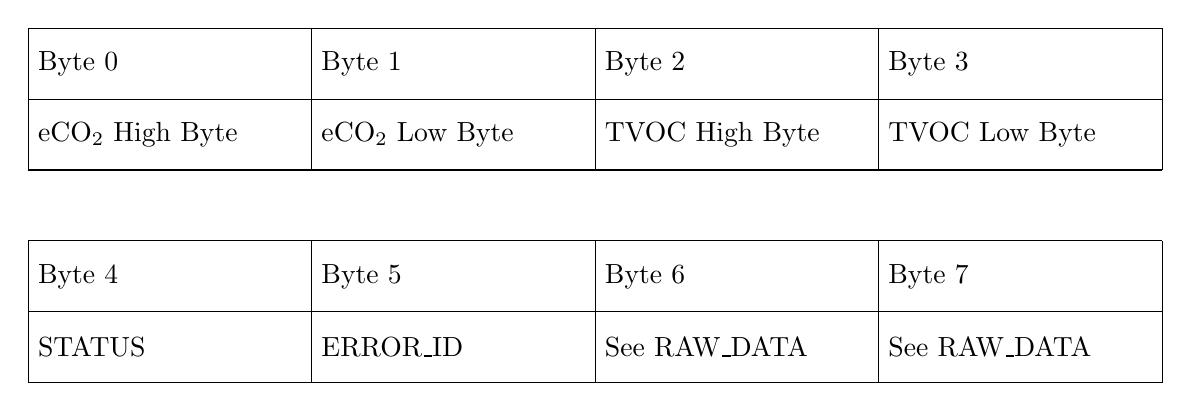
\begin{tikzpicture}[scale=0.9]
		
		
		% Gitter zeichnen (spalte zeile)
		\draw (1,0)--(17,0); 
		\draw (1,1)--(17,1); 
		\draw (1,2)--(17,2);
		
		\draw (1,3)--(17,3);
		\draw (1,4)--(17,4);
		\draw (1,5)--(17,5);
		
		\draw (1,3)--(1,5)node [right,near end]{Byte 0} node[right,near start]{eCO\textsubscript{2} High Byte}; % linke Linie Slave Adress
		\draw (5,3)--(5,5)node [right,near end]{Byte 1} node[right,near start]{eCO\textsubscript{2} Low Byte}; % linke Linie W
		\draw (9,3)--(9,5)node [right,near end]{Byte 2} node[right,near start]{TVOC High Byte};
		\draw (13,3)--(13,5)node [right,near end]{Byte 3} node[right,near start]{TVOC Low Byte};
		\draw (17,3)--(17,5);
		
		
		\draw (1,0)--(1,2)node [right,near end]{Byte 4} node[right,near start]{STATUS};
		\draw (5,0)--(5,2)node [right,near end]{Byte 5} node[right,near start]{ERROR\_ID};
		\draw (9,0)--(9,2)node [right,near end]{Byte 6} node[right,near start]{See RAW\_DATA};
		\draw (13,0)--(13,2)node [right,near end]{Byte 7} node[right,near start]{See RAW\_DATA};
		\draw (17,0)--(17,2);
				
		\end{tikzpicture}
		
		\footnotesize{Quelle: \cite[vgl. S. 14]{amsAG.2016}}
		\caption{Inhalt der 8-Byte-Übertragung des CCS811-\ac{MOX}-Sensors}
		\label{fig:8ByteInfo}
		
	\end{figure}
	
\end{center}


In der Softwareimplementierung wird der Co\textsubscript{2}-Sensor mithilfe der Bibliothek <Ardafruit\_CCS811.h> wie in Abbildung \ref{fig:Setup} gezeigt wird aufgerufen. Zunächst werden Setups für das I$^2$C-Interface und die Hardware durchgeführt. Danach wird geprüft, ob die Kommunikation mit dem Sensor aufgebaut werden kann. Wenn das der Fall ist, wird solange gewartet, bis der Sensor bereit ist, Daten zu lesen. Falls jedoch ein Problem auftritt, wird eine Fehlermeldung ausgegeben und der Arduino geht in eine sogenannte Endlosschleife, bis das Programm neu geladen wird oder der Arduino ausgeschalten wird.

\begin{figure}[!hbt]
	\centering
	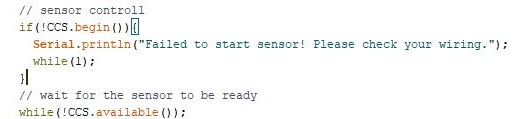
\includegraphics[width=0.9\linewidth]{Images/ccs811Setup}
	\caption{Codeauschnitt im Setup aus dem Softwareprogramm}
	\label{fig:Setup}
\end{figure}

Die Abfrage nach den CO\textsubscript{2}-Werten erfolgt über eine weitere Prüfung auf Fehler und einer anschließenden Messung. Danach werden die Daten auf einem Array gespeichert.

\begin{figure}[!hbt]
	\centering
	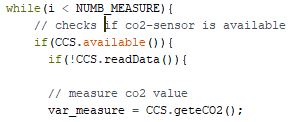
\includegraphics[width=0.5\linewidth]{Images/ccs811Loop}
	\caption{Codeausschnitt für die Messung aus dem Softwareprogramm}
	\label{fig:Loop}
\end{figure}

